\section{Code-Metriken}

\begin{tcolorbox}[title=Code-Metriken]
    Eine andere Herangehensweise für die werkzeuggestützte Analyse stellt die Ermittlung von \textbf{Code-Metriken} dar: Hierbei werden \textbf{Kennzahlen} bestimmt, anhand derer sich die \textbf{Wartbarkeit} von Source-Code beurteilen lässt.\\
    Code-Metriken stehen in \textit{engem Zusammenhang} mit \textbf{Prinzipien guten Entwurfs}.
\end{tcolorbox}
\vspace{2mm}

\begin{figure}
    \centering
    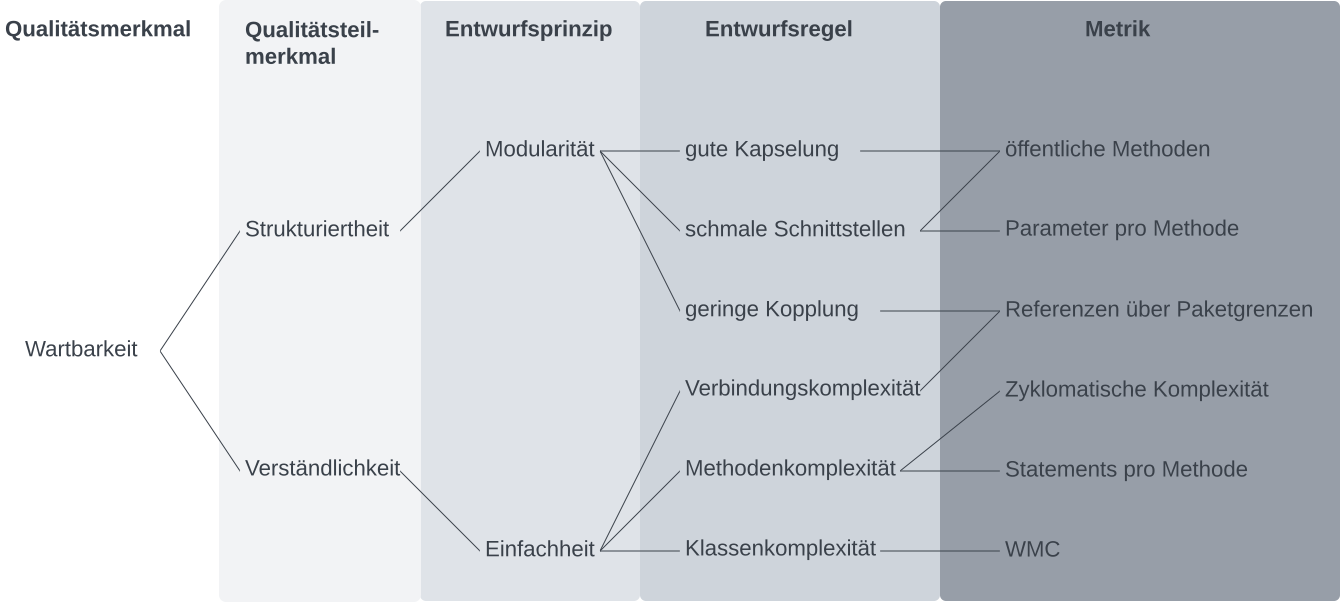
\includegraphics[scale=0.35]{part four/Werkzeuggestützte Analyse/img/metriken}
    \caption{Typische Metriken zur Bestimmung des \textbf{Qualitätsmerkmals} \textit{Wartbarkeit} und ihr Zusammenhang mit den Qualitätsteilmerkmalen. \textbf{WMC} steht für  \textit{Weighted Mean Complexity} (s. ``Komplexität``). (Quelle: in Anlehnung an \cite[Abb. 4.3, 37]{Wed09c})}
    \label{fig:metriken-cc}
\end{figure}